%% -*- coding:utf-8 -*-
\chapter{Base definitions of probability theory}
I am going to provide several definitions. I will give the both formal
and informal definitions and show how they are related each other.

\section{Example and motivation}
We will start with the simplest example. 
\begin{example}
\label{ex:initial}
In the example we have (see \cref{fig:simpleprobability}) $N=5$ balls.
There are $N_G = 2$ green balls and $N_R$ red balls. I.e. $N = N_G +
N_R$.  
\begin{figure}[H]
  \centering
  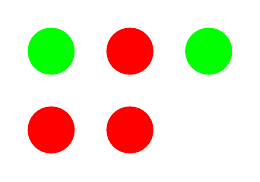
\begin{tikzpicture}[ele/.style={fill=black,circle,minimum
        width=.8pt,inner sep=1pt},every fit/.style={ellipse,draw,inner
        sep=-2pt}]
    \tikzstyle{element}=[circle,fill=black!25,minimum size=17pt,inner sep=0pt]

    \node[element, color=green] at (0,1) {};
    \node[element, color=red] at (1,1) {};
    \node[element, color=green] at (2,1) {};
    \node[element, color=red] at (0,0) {};
    \node[element, color=red] at (1,0) {};


  \end{tikzpicture}
  \caption{Probability example}
  \label{fig:simpleprobability}
\end{figure}

We can define the probability to get green ball as
\[
P_G = \frac{N_G}{N} = \frac{2}{5}
\]
and the probability to get red ball as
\[
P_R = \frac{N_R}{N} = \frac{3}{5}.
\]
We can get only a red or a green ball and 
\[
P_G + P_R = 1.
\]
\end{example}

\section{Definitions}
Now we are ready to give several formal definitions. 
\subsection{$\sigma$-algebra}
\begin{definition}[Power set]
\label{def:powerset}
Let $\Omega$ is a set than the set of all possible subsets of $\Omega$
is called \textit{power set} and denoted as
$\mathcal{P}\left(\omega\right)$. 
\end{definition}

\begin{definition}[$\sigma$ algebra]
Let $\Omega$ is a set then a subset $\mathcal{F}$ of
\mynameref{def:powerset} $\mathcal{P}\left(\Omega\right)$ ($\mathcal{F}\subseteq
\mathcal{P}\left(\Omega\right)$) is called $\sigma$ algebra if the
following conditions are 
satisfied:
\begin{enumerate}
\item $\mathcal{F}$ contains $\Omega$: $\Omega \in \mathcal{F}$
\item TBD
\item TBD
\end{enumerate} 
\end{definition}

In our \cref{ex:initial}, $\sigma$ algebra is a collection of any
balls. 

\begin{figure}
  \centering
  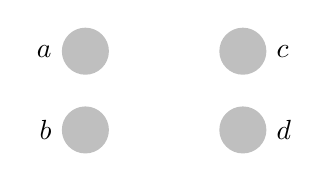
\begin{tikzpicture}[ele/.style={fill=black,circle,minimum
        width=.8pt,inner sep=1pt},every fit/.style={ellipse,draw,inner
        sep=-2pt}]

    % the texts
    \tikzstyle{element}=[circle,fill=black!25,minimum size=17pt,inner
      sep=0pt]

    \node[element,label=left:$a$] (a) at (0,2) {};    
    \node[element,label=left:$b$] (b) at (0,1) {};    
    \node[element,label=right:$c$] (c) at (2,2) {};
    \node[element,label=right:$d$] (d) at (2,1) {};
    
  \end{tikzpicture}
  \caption{Probability space. It consists of elementary events: $a$,
    $b$, $c$ and $d$, each
    of them has equal probability $p_{a,b,c,d} = \frac{1}{4}$}
  \label{fig:probabilityspace}
\end{figure}

\section{Conditional probability}

\begin{definition}[Conditional probability]
\label{def:conditionalprobability}
The \textit{conditional probability} of event $A$ on event $B$ is
defined as follow
\[
P(A|B) = \frac{P\left(A \cap B\right)}{P(B)}
\]
\end{definition}

\begin{example}[Conditional probability]
\label{ex:conditionalprobability}
Lets consider 6 balls each of them can be either two colors (see
\cref{fig:excondprobability}). 
\begin{figure}[H]
  \centering
  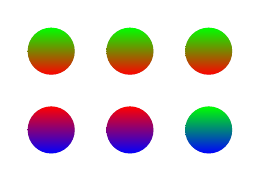
\begin{tikzpicture}[ele/.style={fill=black,circle,minimum
        width=.8pt,inner sep=1pt},every fit/.style={ellipse,draw,inner
        sep=-2pt}]
    \tikzstyle{element}=[circle,fill=black!25,minimum size=17pt,inner sep=0pt]

    \node[element,top color=green, bottom color=red] at (0,1) {};
    \node[element,top color=green, bottom color=red] at (1,1) {};
    \node[element,top color=green, bottom color=red] at (2,1) {};
    \node[element,top color=red, bottom color=blue] at (0,0) {};
    \node[element,top color=red, bottom color=blue] at (1,0) {};
    \node[element,top color=green, bottom color=blue] at (2,0) {};


  \end{tikzpicture}
  \caption{Condition probability. Original probability space. $P(A = red) =
    \frac{5}{6}$, $P(A = blue) = \frac{3}{6}$, $P(A = green) = \frac{4}{6}$
  }
  \label{fig:excondprobability}
\end{figure}
You can see that the probability $P(A)$ to get red ball is $P(A = red) =
\frac{5}{6}$, blue one is $P(A = blue) = \frac{3}{6}$, green one is
$P(A = green) =
\frac{4}{6}$. 

Now assume that event $A$ is to get a green ball but event $B$ is to
get red ball, how we can define $P(A|B)$ in the case. 

\begin{figure}[H]
  \centering
  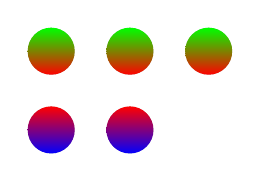
\begin{tikzpicture}[ele/.style={fill=black,circle,minimum
        width=.8pt,inner sep=1pt},every fit/.style={ellipse,draw,inner
        sep=-2pt}]
    \tikzstyle{element}=[circle,fill=black!25,minimum size=17pt,inner sep=0pt]

    \node[element,top color=green, bottom color=red] at (0,1) {};
    \node[element,top color=green, bottom color=red] at (1,1) {};
    \node[element,top color=green, bottom color=red] at (2,1) {};
    \node[element,top color=red, bottom color=blue] at (0,0) {};
    \node[element,top color=red, bottom color=blue] at (1,0) {};


  \end{tikzpicture}
  \caption{Condition probability. $P(A = green|B = red) =
    \frac{3}{5}$, $P(A = blue| B = red) = \frac{2}{5}$}
  \label{fig:excondprobability_red}
\end{figure}
The situation is displayed on \cref{fig:excondprobability_red}. We have only 5
possibilities to choose a ball now instead of 6 in the original case.
This is because we just got an additional information - ``one of the
color should be red''. Only 3 of the 5 balls are green. Therefore
$P(A|B) = P(A=green|B=red) = \frac{3}{5}$. 

This result is in correlation with the formal definition of
\mynameref{def:conditionalprobability}:
\begin{eqnarray}
P(A|B) = \frac{P\left(A \cap B\right)}{P(B)} = 
\nonumber \\
\frac{P\left(A = green \cap B = red\right)}{P(B = red)} = 
\frac{3/6}{5/6} = \frac{3}{5}.
\nonumber
\end{eqnarray}

The \cref{fig:excondprobability_blue} gives as the view if event
$B=blue$ occurs. 
\begin{figure}[H]
  \centering
  
\begin{tikzpicture}[ele/.style={fill=black,circle,minimum
        width=.8pt,inner sep=1pt},every fit/.style={ellipse,draw,inner
        sep=-2pt}]
    \tikzstyle{element}=[circle,fill=black!25,minimum size=17pt,inner sep=0pt]

    \node[element,top color=red, bottom color=blue] at (0,0) {};
    \node[element,top color=red, bottom color=blue] at (1,0) {};
    \node[element,top color=green, bottom color=blue] at (2,0) {};


  \end{tikzpicture} 
  \caption{Condition probability. $P(A = red|B=blue) = \frac{2}{3}$,
    $P(A= green|B = blue) = \frac{1}{3}$} 
  \label{fig:excondprobability_blue}
\end{figure}
In the case we have the following conditional probabilities:
$P(A = red|B=blue) = \frac{2}{3}$, $P(A= green|B = blue) =
    \frac{1}{3}$.

Finally, the \cref{fig:excondprobability_green} gives as the view if event
$B=green$ occurs. 
\begin{figure}[H]
  \centering
  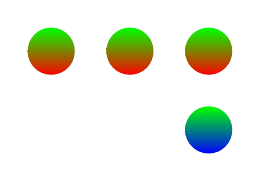
\begin{tikzpicture}[ele/.style={fill=black,circle,minimum
        width=.8pt,inner sep=1pt},every fit/.style={ellipse,draw,inner
        sep=-2pt}]
    \tikzstyle{element}=[circle,fill=black!25,minimum size=17pt,inner sep=0pt]

    \node[element,top color=green, bottom color=red] at (0,1) {};
    \node[element,top color=green, bottom color=red] at (1,1) {};
    \node[element,top color=green, bottom color=red] at (2,1) {};
    \node[element,top color=green, bottom color=blue] at (2,0) {};


  \end{tikzpicture}
  \caption{Condition probability. $P(A = blue|B = green) =
    \frac{1}{4}$, $P(A = red|B = green) =
    \frac{3}{4}$} 
  \label{fig:excondprobability_green}
\end{figure}
\end{example}

\begin{example}[The King's sibling]
Suppose that we have a king from a family of 2 children. What's the
probability that his sibling is a girl. The important assumption
\footnote{
For instance if the king family assume to get a new child until the
first boy (king) get then we will have the sibling is girl with
probability $1$.
}
that
has to be made is the following: there is no any family planning in
the king family and the probability to get a boy $P_b$ and probability
to get a girl $P_b$ are equally likely:
\[
P_b = P_g = \frac{1}{2}.
\] 
We have 4 cases: $bb, bg, gb, gg$ and the condition that the king is a
boy pick up only 3 options for us: $bb, bg, gb$. All of them are
equally likely and 2 have a girl as sibling. I.e.
\[
P(sibling = girl|king) = \frac{2}{3}.
\]
\end{example}

\begin{proposition}[Total probability]

The \textit{total probability} is defined as follows
\[
P(A) = \sum_i P(A|B_i)
\]
\label{thm:totalprobability}
\end{proposition}

\begin{example}[Total probability]
Lets assume in the \mynameref{ex:conditionalprobability} that we are
interested in the event $A$ that the ball is green. The other color
will be either blue or red. I.e. $B_1 = blue$, $B_2 = red$.
\begin{eqnarray}
P(A = green) = P(A = green|B = blue) P(B = blue) +
\nonumber \\
+
P(A = green|B = red) P(B = red) =
\nonumber \\
= \frac{1}{3} \cdot \frac{1}{2} + \frac{3}{5}\cdot \frac{5}{6} = \frac{4}{6}.
\nonumber
\end{eqnarray}
I.e. formula works.
\end{example}

Consider another, not so simple example
\begin{example}[Total probability paradox]
Let we have 6 balls each of them has one color: red or green (see
\cref{fig:excondprobability_add}). 
\begin{figure}[H]
  \centering
  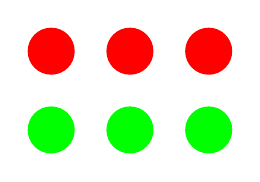
\begin{tikzpicture}[ele/.style={fill=black,circle,minimum
        width=.8pt,inner sep=1pt},every fit/.style={ellipse,draw,inner
        sep=-2pt}]
    \tikzstyle{element}=[circle,fill=black!25,minimum size=17pt,inner sep=0pt]

    \node[element,color=red] at (0,1) {};
    \node[element,color=red] at (1,1) {};
    \node[element,color=red] at (2,1) {};
    \node[element,color=green] at (0,0) {};
    \node[element,color=green] at (1,0) {};
    \node[element,color=green] at (2,0) {};


  \end{tikzpicture}
  \caption{Total probability example}
  \label{fig:excondprobability_add}
\end{figure}
Lets event $A$ is an event to get a ball. $P(A) = \frac{1}{6}$. The
event $B_1$ is an event to get green ball: $P(B_1) = \frac{1}{2}$. The
same one is for probability to get red ball: $P(B_2) = \frac{1}{2}$.
Conditional probabilities can be calculated as follows:
\begin{equation}
P(A|B_1) = P(A|B_2) = \frac{1}{3}.
\label{eq:condprob_wrong}
\end{equation}
As result the total probability is 
\[
P(A) = \frac{1}{2}\cdot\frac{1}{3} + \frac{1}{2}\cdot\frac{1}{3} =
\frac{2}{6} \ne \frac{1}{6}.
\]
The error is in the \eqref{eq:condprob_wrong}. When we consider a
concrete ball then it either green or blue and as result one of the
conditional probabilities $P(A|B_1)$ or $P(A|B_2)$ is zero. In the
case we will get correct answer $P(A) = \frac{1}{6}$.
\end{example}

\begin{definition}[Independence]
\label{def:independence}
Two events $A$ and $B$ are independent if 
\[
P\left(A \cap B\right) = 
P\left(A\right) P\left(B\right). 
\]
\end{definition}

\begin{example}[Non independent events]
Consider situation shown in \cref{fig:excondprobability_add}. Let
event $A$ is that ball is green, event $B$ is that ball is red. We
have
\[
A \cap B = \emptyset, 
\]
i.e. $P\left(A \cap B\right) = 0$. This means that the events cannot
be considered as independent accordingly \cref{def:independence} as
soon as $P\left(A\right) = 
P\left(B\right) = \frac{1}{2}$.

Really the events are dependent as soon as we can say that $A$ will
not occur if $B$ occurs and vice versa.
\end{example}

\begin{example}[Fish in a pond]
The example from a Russian Biological Olympiad. Consider a pond with
fishes. 15 of them were marked. After sometime we took 15 fishes and 5
of them were marked. How many fishes in the pond.

The accepted answer was 45 with the following explanation: 
\[
\frac{15}{5} = \frac{n}{15}
\]
therefore $n=45$.

Lets try to solve the task with probability theory and convert the
question to the following one: In every 15 fishes with max probability
we find 5 marked ones. How many fishes in the pond.

The probability to get a marked fish is
\[
P_1 = \frac{15}{n}
\]
but if we catch a fish then the probability (conditional) to get a new
marked fish is
\[
P_2 = \frac{14}{n-1}
\]
i.e. the probability to catch $i$-th marked fish is
\[
P_i = \frac{15-i+1}{n - i + 1}.
\]
The probability to catch the first non marked fish is
\[
Q_1 = \frac{n - 15}{n - 5},
\]
$i$-th
\[
Q_i = \frac{n -15 -i + 1}{n - 5 - i + 1}
\]
The final probability is
\[
P = \frac{\prod_{k=11}^{15}k}{\prod_{i = 1}^{15}{\left(n - 15 - i +
    1\right)}}\prod_{k=1}^{10}{\left(n -k + 1\right)}.
\]

Quick calculations show that $n=45$ is very close to real answer: 
\begin{verbatim}
Prelude> p1 n = foldl (\x y -> x * (n - y)) 1 [0 .. 14]
Prelude> p2 n = foldl (\x y -> x * (n - 15 - y)) 1 [0 .. 9]
Prelude> fn n = (product [11 .. 15])*(p2 n)/(p1 n)
Prelude> map fn [50, 45, 35, 30, 25, 20]
[8.156077120597312e-5,8.7120478105816e-5,5.688400039611531e-5,
1.935951528879523e-5,3.0592640634368994e-7,0.0]
Prelude> 
\end{verbatim}

\end{example}

TBD \cite{bib:kolmogorov74basic}
